\documentclass[tikz, border=2pt]{standalone}
\usepackage{tikz}
\usetikzlibrary{shapes,arrows,positioning,calc}

% ==========================================
% STYLES
% ==========================================
\tikzstyle{process} = [rectangle, draw, fill=black!3, rounded corners,
  text width=8em, text centered, minimum height=1.5em, font=\small]
\tikzstyle{decision} = [rectangle, draw, fill=orange!3, rounded corners,
  text width=8em, text centered, minimum height=1.5em, font=\small]
\tikzstyle{file} = [cylinder, draw, fill=blue!4,
  minimum width=1.4cm, minimum height=0.28cm, font=\footnotesize,
  cylinder uses custom fill, cylinder body fill=blue!3, cylinder end fill=blue!6]
\tikzstyle{snode} = [rectangle, draw, fill=black!3, rounded corners,
  text width=6em, text centered, minimum height=1.5em, font=\small]
\tikzstyle{final} = [rectangle, draw=green!50!black, line width=1.2pt,
  fill=green!2, rounded corners, text width=6cm, text centered,
  minimum height=1.8em, font=\small]
\tikzstyle{ann} = [font=\scriptsize, text=black!50, text width=7.5em, align=left,
  fill=white, inner sep=2pt]
\tikzstyle{cite} = [font=\scriptsize\itshape, text=green!35!black]
\tikzstyle{line} = [draw, -latex', thick]

\begin{document}
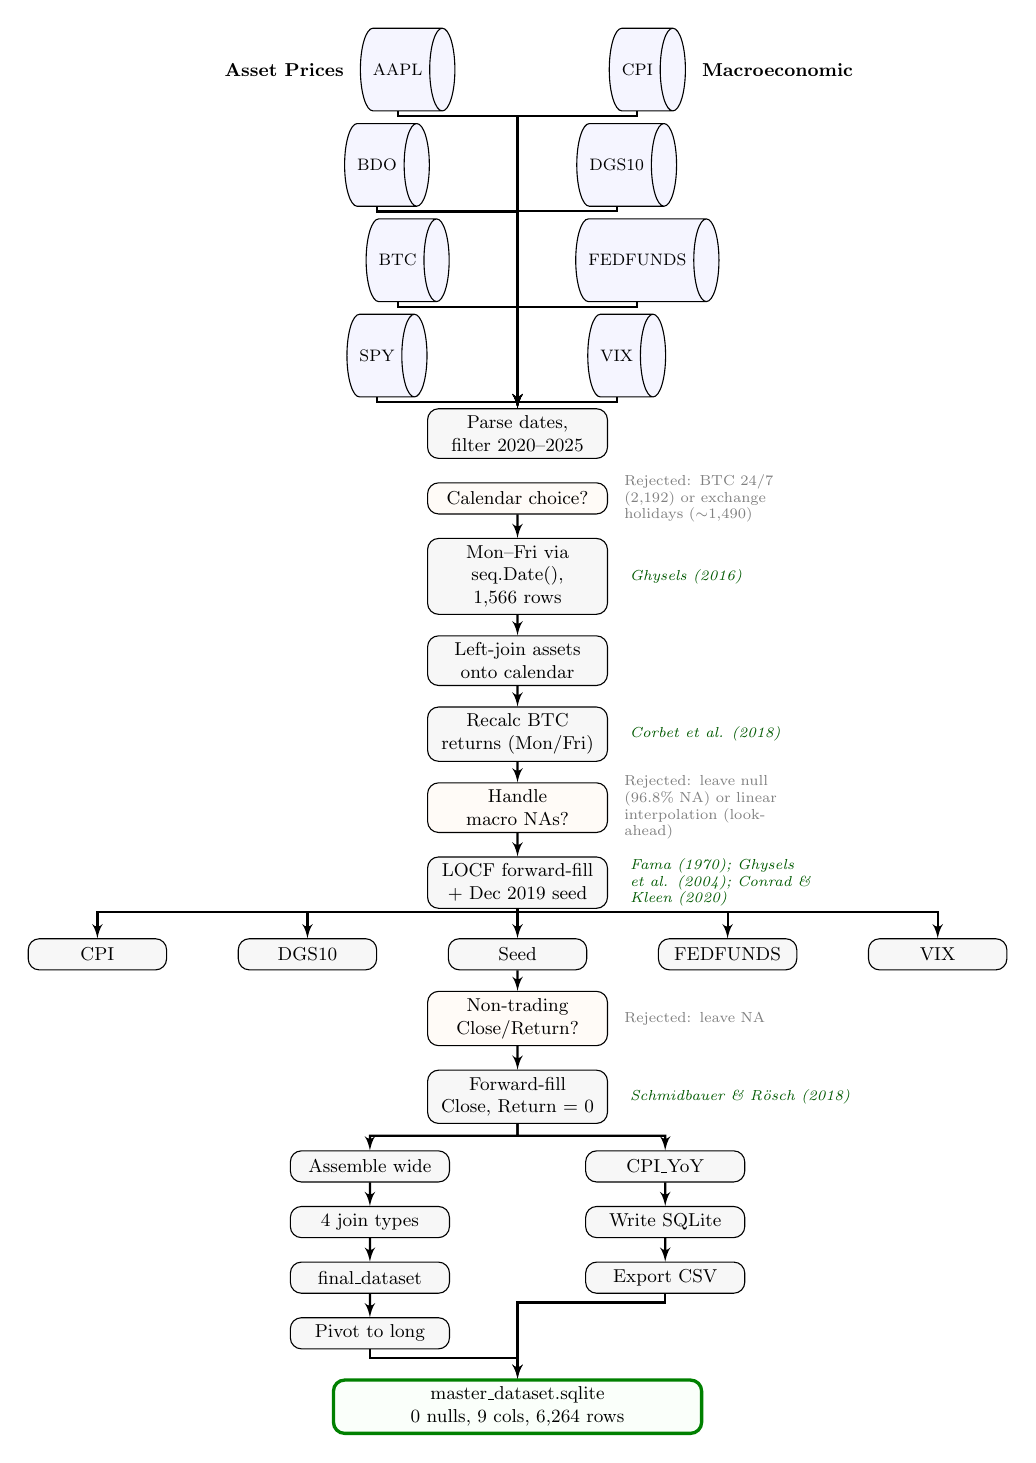
\begin{tikzpicture}[scale=0.75, transform shape, node distance=0.35cm, auto, >=stealth]

% ==========================================
% ASSET PRICES CLUSTER (left column)
% ==========================================
\node[file] (aapl) {AAPL};
\node[file] (bdo)  [below=0.2cm of aapl, xshift=-0.35cm] {BDO};
\node[file] (btc)  [below=0.2cm of bdo, xshift=0.35cm]  {BTC};
\node[file] (spy)  [below=0.2cm of btc, xshift=-0.35cm] {SPY};

% ==========================================
% MACROECONOMIC CLUSTER (right column)
% ==========================================
\node[file] (cpi) [right=2.6cm of aapl] {CPI};
\node[file] (dgs10) [below=0.2cm of cpi, xshift=-0.35cm] {DGS10};
\node[file] (fedfunds) [below=0.2cm of dgs10, xshift=0.35cm] {FEDFUNDS};
\node[file] (vix) [below=0.2cm of fedfunds, xshift=-0.35cm] {VIX};

% Column labels -- outer sides
\node[font=\small\bfseries, left=0.15cm of aapl, anchor=east] (asset_label) {Asset Prices};
\node[font=\small\bfseries, right=0.15cm of cpi, anchor=west] (macro_label) {Macroeconomic};

% Central anchor
\path (btc.south) -- (fedfunds.south) coordinate[midway] (center_anchor);

% ==========================================
% LAYER 2: Parse & Filter
% ==========================================
\node[process] (parse) [below=1.8cm of center_anchor] {Parse dates, filter 2020--2025};
\foreach \f in {aapl,bdo,btc,spy,cpi,dgs10,fedfunds,vix}
  { \draw[line] (\f.south) -- ++(0, -0.08) -| (parse.north); }

% ==========================================
% LAYER 3: Calendar
% ==========================================
\node[decision] (cal_q) [below=0.4cm of parse] {Calendar choice?};
\node[ann, right=0.2cm of cal_q, anchor=west] {Rejected: BTC 24/7 (2,192) or exchange holidays ($\sim$1,490)};
\node[process] (cal) [below=0.4cm of cal_q] {Mon--Fri via seq.Date(), 1,566 rows};
\node[cite, right=0.25cm of cal, anchor=west] {Ghysels (2016)};
\draw[line] (cal_q.south) -- (cal.north);

% ==========================================
% LAYER 4: Join & Return
% ==========================================
\node[process] (join) [below=0.35cm of cal] {Left-join assets onto calendar};
\draw[line] (cal.south) -- (join.north);
\node[process] (btc_r) [below=0.35cm of join] {Recalc BTC returns (Mon/Fri)};
\node[cite, right=0.25cm of btc_r, anchor=west] {Corbet et al. (2018)};
\draw[line] (join.south) -- (btc_r.north);

% ==========================================
% LAYER 5: Macro forward-fill
% ==========================================
\node[decision] (mq) [below=0.35cm of btc_r] {Handle macro NAs?};
\node[ann, right=0.2cm of mq, anchor=west] {Rejected: leave null (96.8\% NA) or linear interpolation (look-ahead)};
\node[process] (mfill) [below=0.4cm of mq] {LOCF forward-fill + Dec 2019 seed};
\node[cite, right=0.25cm of mfill, anchor=west, text width=10em, align=left] {Fama (1970); Ghysels et al. (2004); Conrad \& Kleen (2020)};
\draw[line] (btc_r.south) -- (mq.north);
\draw[line] (mq.south) -- (mfill.north);

% Macro sub-nodes
\node[snode] (ff3) [below=0.5cm of mfill] {Seed};
\node[snode] (ff2) [left=1.2cm of ff3] {DGS10};
\node[snode] (ff1) [left=1.2cm of ff2] {CPI};
\node[snode] (ff4) [right=1.2cm of ff3] {FEDFUNDS};
\node[snode] (ff5) [right=1.2cm of ff4] {VIX};
\foreach \x in {ff1,ff2,ff3,ff4,ff5}
  { \draw[line] (mfill.south) -- ++(0, -0.05) -| (\x.north); }

% ==========================================
% LAYER 6: Asset forward-fill
% ==========================================
\node[decision] (aq) [below=0.35cm of ff3] {Non-trading Close/Return?};
\node[ann, right=0.2cm of aq, anchor=west] {Rejected: leave NA};
\node[process] (afill) [below=0.4cm of aq] {Forward-fill Close, Return = 0};
\node[cite, right=0.25cm of afill, anchor=west] {Schmidbauer \& R\"{o}sch (2018)};
\draw[line] (ff3.south) -- (aq.north);
\draw[line] (aq.south) -- (afill.north);

% ==========================================
% LAYER 7: Parallel columns
% ==========================================
% Left branch
\node[snode, text width=7em] (wide) [below=0.45cm of afill, xshift=-2.5cm] {Assemble wide};
\node[snode, text width=7em] (j4)   [below=0.4cm of wide] {4 join types};
\node[snode, text width=7em] (fwd)  [below=0.4cm of j4]  {final\_dataset};
\node[snode, text width=7em] (long) [below=0.4cm of fwd] {Pivot to long};
\draw[line] (afill.south) -- ++(0, -0.2) -- ++(-2.5, 0) -- (wide.north);
\draw[line] (wide) -- (j4);
\draw[line] (j4) -- (fwd);
\draw[line] (fwd) -- (long);

% Right branch
\node[snode, text width=7em] (yoy) [below=0.45cm of afill, xshift=2.5cm] {CPI\_YoY};
\node[snode, text width=7em] (sql) [below=0.4cm of yoy] {Write SQLite};
\node[snode, text width=7em] (csv) [below=0.4cm of sql] {Export CSV};
\draw[line] (afill.south) -- ++(0, -0.2) -- ++(2.5, 0) -- (yoy.north);
\draw[line] (yoy) -- (sql);
\draw[line] (sql) -- (csv);

% ==========================================
% LAYER 8: Final
% ==========================================
\node[final] (fin) [below=0.5cm of long, xshift=2.5cm] {master\_dataset.sqlite\\0 nulls, 9 cols, 6,264 rows};
\draw[line] (long.south) -- ++(0, -0.15) -| (fin.north);
\draw[line] (csv.south) -- ++(0, -0.15) -| (fin.north);

\end{tikzpicture}
\end{document}
